% ============================================================
% !TeX root = ../main.tex
%  Appendix A — Supplementary Methodological Details
% ============================================================
\selectlanguage{english}
\chapter{Supplementary Methodological Details}
\label{app:supplementary-methods}

\noindent
This appendix summarises the training data streams and partitions,
RBF-derived clinical supervision meshes, training-loss terms, and model
configuration described in~\cref{ch:methodology}.

\section{Training Data Streams}
\label{sec:appendix-training-streams}
\noindent
Synthetic meshes establish a geometric shape prior during pre-training;
clinical MRI data support fine-tuning on end-diastolic and end-systolic anatomy.

\begin{table}[H]
	\centering
	\caption[Training data streams and their roles]{Training data streams and their roles.}
	\label{tab:method-datasets}
	\thesistablestyle
	\begin{tabular*}{\textwidth}{@{\extracolsep{\fill}}p{0.17\textwidth} p{0.08\textwidth} p{0.28\textwidth} p{0.31\textwidth}@{}}
		\toprule
		Stream & Phase & Source & Training role \\
		\midrule
		Synthetic SSM & ED & UK Digital Heart Project LV SSM & Pre-training to establish a geometric shape prior \\
		Real MRI & ED & ACDC and M\&Ms-2 & Fine-tuning on patient-specific diastolic anatomy \\
		Real MRI & ES & ACDC and M\&Ms-2 & Fine-tuning on systolic anatomy with phase conditioning \\
		\bottomrule
	\end{tabular*}
\end{table}

\clearpage
\section{Dataset Composition and Partitions}
\label{sec:appendix-dataset-partitions}
\noindent
Clinical samples are divided into training, validation, and test partitions,
while accepted synthetic meshes are reserved for pre-training.

\begin{figure}[H]
	\centering
	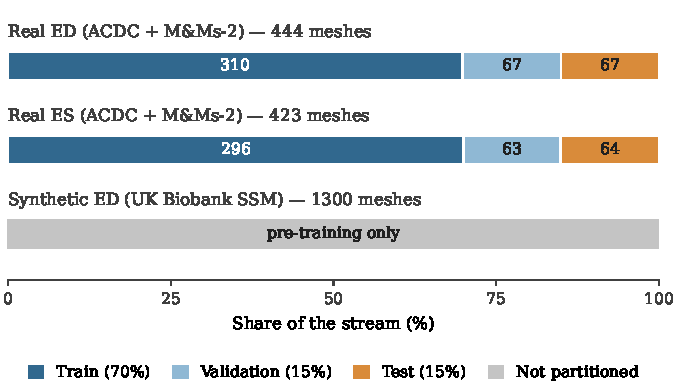
\includegraphics[width=\linewidth,height=0.65\textheight,keepaspectratio]{dataset_selection_and_splits}
	\caption[Composition and splits of the training data streams]{Valid clinical
	samples divided into the 70\,\%/15\,\%/15\,\% partitions. The 1300 accepted
	synthetic meshes are reserved for pre-training.}
	\label{fig:dataset-selection-splits}
\end{figure}

\clearpage
\section{Clinical Mesh Preparation}
\label{sec:appendix-clinical-meshes}
\noindent
The clinical supervision meshes are constructed from SAX contours using
RBF interpolation, surface extraction, and geometric validation.

\begin{table}[H]
	\centering
	\caption[Clinical mesh-preparation operations]{Operations used to construct
	the RBF-derived clinical supervision meshes.}
	\label{tab:real-pipeline}
	\thesistablestyle
	\begin{tabular*}{\textwidth}{@{\extracolsep{\fill}}p{0.34\textwidth} p{0.59\textwidth}@{}}
		\toprule
		Operation & Purpose \\
		\midrule
		RAS+ canonicalisation & Standardises patient-coordinate orientation while preserving physical spacing \\
		Label harmonisation & Maps ACDC and M\&Ms-2 labels to common endocardial and epicardial definitions \\
		Largest-ring extraction and resampling & Retains 60 ordered points per boundary on each acquired SAX slice \\
		In-plane normal estimation & Defines an outward direction at every contour point \\
		Off-surface constraints at $\pm2.5$~mm & Establishes the sign and local scale of each implicit field \\
		Thin-plate-spline RBF fit & Interpolates a continuous field with degree 1 and regularisation parameter 0.5 \\
		Evaluation on a 1.0~mm grid & Discretises the continuous field for surface extraction \\
		Signed-distance regularisation ($\sigma=1.2$~mm) & Reduces voxel-scale corrugation before surface extraction \\
		Connected-region filtering and marching cubes & Removes invalid regions and extracts the zero level set \\
		Topology validation and conditional correction & Preserves valid RBF surfaces and corrects only failed shells \\
		Geometric plausibility checks & Rejects failed fits and invalid endocardial--epicardial pairs \\
		\bottomrule
	\end{tabular*}
\end{table}

\clearpage
\section{Training-Loss Terms}
\label{sec:appendix-training-losses}
\noindent
The five loss terms combine surface and volumetric supervision with
signed-distance regularisation and constraints on the decoder wall offset.

\begin{table}[H]
	\centering
	\caption[Training-loss terms]{Purpose of the five training-loss terms.}
	\label{tab:loss-terms}
	\thesistablestyle
	\begin{tabular*}{\textwidth}{@{\extracolsep{\fill}}p{0.16\textwidth} p{0.34\textwidth} p{0.38\textwidth}@{}}
		\toprule
		Term & Purpose & Effect on reconstruction \\
		\midrule
		$\mathcal{L}_{\mathrm{surf}}$ & Fits zero-level sets to surface samples & Places endocardial and epicardial surfaces on the target meshes \\
		$\mathcal{L}_{\mathrm{SDF}}$ & Fits cached query-point distances & Provides dense volumetric supervision \\
		$\mathcal{L}_{\mathrm{eik}}$ & Encourages $\lVert \nabla f \rVert = 1$ & Regularises the decoder as a signed-distance field \\
		$\mathcal{L}_{\mathrm{off}}$ & Repels off-surface points from zero & Reduces spurious zero crossings away from the myocardium \\
		$\mathcal{L}_{\mathrm{WT}}$ & Fits the predicted wall offset to wall targets & Constrains separation of the predicted fields \\
		\bottomrule
	\end{tabular*}
\end{table}

\clearpage
\section{Model Configuration}
\label{sec:appendix-model-configuration}
\noindent
The configuration below specifies the contour conditioning, decoder
architecture, output fields, and inference grid used by the model.

\begin{table}[H]
	\centering
	\caption[Model architecture settings]{Main architecture settings of the
	model.}
	\label{tab:model-hyperparameters}
	\thesistablestyle
	\begin{tabular*}{\textwidth}{@{\extracolsep{\fill}}p{0.30\textwidth} p{0.63\textwidth}@{}}
		\toprule
		Component & Configuration \\
		\midrule
		Input features & 3D coordinates, tissue label, and cardiac phase \\
		Global encoder type & Shared network with endocardial and epicardial max-pooling \\
		Local conditioning & Coarse 3D contour feature volume with trilinear interpolation \\
		Latent dimension & 256 \\
		Local volume size & $16^3$ with 32 channels \\
		Positional encoding & Fourier features with $L=3$ frequency bands \\
		Decoder & 8-layer network, width 512, skip connection at layer 4 \\
		Activation & Softplus (smooth) \\
		Local injections & Local feature paths into the decoder trunk and offset head \\
		Output heads & Endocardial signed distance and positive decoder wall-offset field \\
		Offset mapping & Sigmoid component with $\tau_{\min}=0.05$ and $\delta_{\mathrm{cap}}=0.45$, plus learned soft-hinge headroom \\
		Inference grid & $96^3$ query grid for marching cubes \\
		\bottomrule
	\end{tabular*}
\end{table}

\clearpage
\section{Training Configuration}
\label{sec:appendix-training-configuration}
\noindent
The settings below specify the optimisation, schedule, batching, and hardware
used to train the model in both stages.

\begin{table}[H]
	\centering
	\caption[Model training configuration]{Training configuration used for the
	model.}
	\label{tab:training-config}
	\thesistablestyle
	\begin{tabular*}{\textwidth}{@{\extracolsep{\fill}}p{0.30\textwidth} p{0.63\textwidth}@{}}
		\toprule
		Setting & Value \\
		\midrule
		Training strategy & SSM pre-training, then fine-tuning on real ED/ES \\
		Training mode & Combined ED and ES with phase conditioning \\
		Augmentation & Contour-input perturbations for synthetic ED and real ED/ES; targets unchanged \\
		Optimiser & AdamW \\
		Learning rate & $2\times10^{-5}$ \\
		Scheduler & Cosine annealing with warm restarts ($T_0=100$ epochs) \\
		Weight decay & $5\times10^{-4}$ \\
		Training duration & Approximately 200 pre-training epochs, then 776 fine-tuning epochs (best checkpoint: 695) \\
		Batch size & 8 per GPU $\times$ 2 GPUs, accumulated for 2 steps (effective batch size 32) \\
		Gradient clipping & 1.0 \\
		Precision & Automatic mixed precision \\
		Hardware & 2 GPUs in parallel \\
		Inference grid & $96^3$ \\
		\bottomrule
	\end{tabular*}
\end{table}
